\chapter{Results}
\label{chap:results}

This chapter will present some results from simulating the lottery being set up and played. We primarily measure gas usage, which is the same on the local blockchain used for simulations as the main live Ethereum blockchain used in production. The transaction costs on Ethereum are measured in each transaction's gas usage. The transaction costs, which will be used interchangeably with gas costs, is the product of the gas usage and a gas price. The gas usage is a unitless number, while the gas price is denominated in \emph{wei}, which is the most granular unit of ether. $1 wei=1 \mathrm{e}{-18} ether$. It's common to quote the gas price in gwei, which is simply a gigawei ($1\mathrm{e}{9} wei$). When quoting prices in USD we operate with an ether price of 176 USD. Unless otherwise stated, a gas price of 1.5 gwei is used in calculations. This is a quite low gas price, but usually high enough to have transactions included in the blockchain within 30 minutes or so.

In addition to presenting the results from simulation, we will analyze the security and scalability of the lottery. Some calculations will be made where both the gas usage results from the simulations and reasonable assumptions of gas price and maximum lottery prize will be used.
The last section of the chapter will discuss the consequences of our design choices and trade-offs for the properties of the lottery, and suggest some alternative designs that will result in a lottery with different properties.

\section{Gas usage and transaction costs}
\label{sec:gas}

\begin{table}[h]
\centering
\caption{Average gas usage from simulation.}
\label{tab:gas-usage}
\begin{tabular}{|l|l|l|l|}
\hline

transaction & single match & dual match & \# \\ \hline
create LotteryMaster & 1087189 & 1087125 & 1 \\ \hline
setFinalMatch & 49282 & 49282 & 1 \\ \hline
create LotteryMatch & 2472237 & - & N-1 \\ \hline
create FirstLevelMatch & - & 1693728 & N/2 \\ \hline
create InternalMatch & - & 1697819 & (N/2)-1 \\ \hline
initFirstLevelMatch & 74700 & - & N/2 \\ \hline
initInternalMatch & 71034 & - & (N/2)-1 \\ \hline
deposit & 73925 & 73925 & N \\ \hline
commit & 83548 & 88668 & 2(N-1) \\ \hline
reveal & 43035 & 42882 & 2(N-1) \\ \hline
withdraw & 39277 & 39177 & 1 \\ \hline

\end{tabular}
\end{table}

\noindent
Table \ref{tab:gas-usage} is a list of transactions made in a simulation with 256 participants. The left column describes the transaction made, while the right column is the number of transactions of this type needed to successfully play a lottery. The middle columns are the average gas usage for each transaction for two different lottery designs. In the first design, we use a single match contract for all types of matches whether they are first level or internal. In the second design, we have two separate match contracts for first level matches and internal matches. 

\begin{table}[h]
\centering
\caption{Organizer gas usage. Single match contract.}
\label{tab:org-gas-usage-single}
\begin{tabular}{|l|l|l|l|l|l|l|l|}
\hline

N & Gas & ETH & USD & Gas / N & ETH / N & USD / N & $\Delta$ Gas / N \\ \hline
32 & 80023408 & 0.120 & 21.13 & 2500732 & 0.003751 & 0.660 &  \\ \hline
64 & 161466448 & 0.242 & 42.63 & 2522913 & 0.003784 & 0.666 & 22182 \\ \hline
128 & 324354704 & 0.487 & 85.63 & 2534021 & 0.003801 & 0.669 & 11108 \\ \hline
256 & 650139920 & 0.975 & 171.64 & 2539609 & 0.003809 & 0.670 & 5588 \\ \hline
512 & 1301701456 & 1.953 & 343.65 & 2542386 & 0.003814 & 0.671 & 2777 \\ \hline

\end{tabular}
\end{table}

\begin{table}[h]
\centering
\caption{Total gas usage. Single match contract.}
\label{tab:total-gas-usage-single}
\begin{tabular}{|l|l|l|l|l|l|l|l|}
\hline

N & Gas & ETH & USD & Gas / N & ETH / N & USD / N & $\Delta$ Gas / N \\ \hline
32 & 90297000 & 0.135 & 23.84 & 2821781 & 0.004233 & 0.745 &  \\ \hline
64 & 182203802 & 0.273 & 48.10 & 2846934 & 0.004270 & 0.752 & 25153 \\ \hline
128 & 366020720 & 0.549 & 96.63 & 2859537 & 0.004289 & 0.755 & 12602 \\ \hline
256 & 733661484 & 1.100 & 193.69 & 2865865 & 0.004299 & 0.757 & 6328 \\ \hline
512 & 1468940796 & 2.203 & 387.80 & 2869025 & 0.004304 & 0.757 & 3160 \\ \hline

\end{tabular}
\end{table}

\begin{table}[h]
\centering
\caption{Organizer gas usage. Two types of match contracts.}
\label{tab:org-gas-usage-dual}
\begin{tabular}{|l|l|l|l|l|l|l|l|}
\hline

N & Gas & ETH & USD & Gas / N & ETH / N & USD / N & $\Delta$ Gas / N \\ \hline
32 & 53690344 & 0.081 & 14.17 & 1677823 & 0.002517 & 0.443 &  \\ \hline
64 & 107956984 & 0.162 & 28.50 & 1686828 & 0.002530 & 0.445 & 9005 \\ \hline
128 & 216490200 & 0.325 & 57.15 & 1691330 & 0.002537 & 0.447 & 4502 \\ \hline
256 & 433556696 & 0.650 & 114.46 & 1693581 & 0.002540 & 0.447 & 2251 \\ \hline
512 & 867690392 & 1.302 & 229.07 & 1694708 & 0.002542 & 0.447 & 1127 \\ \hline

\end{tabular}
\end{table}

\begin{table}[h]
\centering
\caption{Total gas usage. Two types of match contracts.}
\label{tab:total-gas-usage-dual}
\begin{tabular}{|l|l|l|l|l|l|l|l|}
\hline

N & Gas & ETH & USD & Gas / N & ETH / N & USD / N & $\Delta$ Gas / N \\ \hline
32 & 63896706 & 0.096 & 16.87 & 1996772 & 0.002995 & 0.527 &  \\ \hline
64 & 128557218 & 0.193 & 33.94 & 2008707 & 0.003013 & 0.530 & 11934 \\ \hline
128 & 257880692 & 0.387 & 68.08 & 2014693 & 0.003022 & 0.532 & 5986 \\ \hline
256 & 516523956 & 0.775 & 136.36 & 2017672 & 0.003027 & 0.533 & 2979 \\ \hline
512 & 1033816570 & 1.551 & 272.93 & 2019173 & 0.003029 & 0.533 & 1501 \\ \hline

\end{tabular}
\end{table}

\noindent
Table \ref{tab:org-gas-usage-single} and \ref{tab:total-gas-usage-single} show the gas usage of only setting up and setting and playing a full lottery, respectively, for the design with a single type of match contract. Table \ref{tab:org-gas-usage-dual} and \ref{tab:total-gas-usage-dual} show the gas usage for the design with two types of match contracts, also showing for only setting up and setting up and playing a full lottery.
The dual match design compared to the single match design uses 50\% less gas to set up, and 42\% less gas to set up and play. As we can see in Table \ref{tab:gas-usage}, the savings come from deploying the match contracts. This is because we deploy less bytecode and declare fewer variables with the dual match design.

As was expected, the gas usage increases linearly with the number of participants. Even though the gas per participant also increases by a minuscule amount as the number of participants grow, this amount goes towards zero with more participants. For simulating the entire lifecycle of a lottery, this can be explained by the \texttt{deposit()} function which keeps expanding a dynamic array as players join. We will use the measurements for dual matches from Table \ref{tab:gas-usage} in calculations later in this chapter to analyze ticket pricing and scalability. By using the amount of transactions necessary of each type, we see that the gas usage for a lottery of $N$ players can be expressed as for just setting up the lottery $\frac{3391547 \cdot N}{2} - 561412$ and $\frac{4065677 \cdot N}{2} - 785375$ for setting up and playing the entire lottery.

The bulk of the transaction costs of a lottery is setting up all the contracts, which must be done by the lottery organizer. The setup cost is 84\% of the total transaction costs for the 512 player simulation for dual match contracts. We see that by far most gas is spent on deploying each individual match contract. This cost was significantly decreased by splitting the match contracts into two types, the \texttt{FirstLevelMatch} and \texttt{InternalMatch}. This is because each variable and each bit of bytecode contributes to the gas usage when deploying contracts. Decreasing the number of methods, decreasing the number and size of variables, and decreasing the number of instructions, i.e. lines of code, will decrease the gas usage. Since each match contract is not interacted with much – at most four times, two commits and two reveals – it seems wasteful to spend so much gas on deploying them on the blockchain permanently. This is a well-known issue, and it is possible to deduplicate common behaviour by using patterns involving \emph{library contracts} and \emph{proxy contracts}. \cite{lu_solidity_2018} demonstrate that gas usage for deploying contracts can decrease as much as 50\% by using these patterns. It could also be possible to do away with the dedicated match contracts completely, and handle everything in the master contract, but we leave that to future work or a practical implementation.

While the price of ether and by extension gas is known to fluctuate heavily in fiat currency terms, we choose to primarily consider the cost of running the lottery only in the context of ether and gas price, even though we will also mention the price in USD in some cases to provide context. The transaction costs depend entirely on gas usage and gas price, and can be made an arbitrarily low fraction of the ticket price if we can set the ticket price arbitrarily high. The gas price is also known for fluctuating somewhat in terms of ether, but it is simply a result of market demand for resources on the EVM. The gas price is not a fixed price, as there is essentially a bid and ask market with a spread, where transactors are bidders and miners are askers. By bidding with a low gas price, it means the probability of the transaction being included in a block is low, as miners are likely to include transactions with a higher gas price.

\section{Ticket price}
\label{sec:ticket-price}

We operate with a gas price of 1.5 gwei, which at the time of writing is considered quite low, but still enough to make the transaction be included in about 30 minutes or so. Gas prices in Ethereum are denominated in \emph{wei}, which is the most granular unit of ether. $1 wei=1 \mathrm{e}{-18} ether$. A gwei is simply a gigawei ($1\mathrm{e}{9} wei$). When quoting prices in USD we operate with an ether price of 176 USD. 

Most common casino games have a house edge of about 1-10\%~\cite{walsh_houses_nodate}, while large lotteries often have a higher house edge of 40-50\%~\cite{shackleford_house_nodate}. We therefore consider the organizer taking a 10\% fee of the deposits reasonable for both the players and the organizer. The organizer risks not enough players joining the lottery and thus losing all the ether needed to set up the lottery. 

By setting a ratio $r$ of what the organizer will take of the prize, and a gas price $price_{gas}$, we can find a minimum ticket price $price_{ticket}$ by using the gas usage $usage_{gas}$ from Table \ref{tab:org-gas-usage-dual} for setting up the lottery per player. The expression is simply $price_{ticket}=\frac{price_{gas} \cdot usage_{gas}}{r}$
In our design, a 10\% organizer fee and a 1.5 gwei gas price, this results in a minimum viable price of each ticket at about 0.026 ether, which at the time of writing is about 5 USD. That's a price we consider acceptable, even though the dollar price can change by at least an order of magnitude within months, as the ether price fluctuates a lot. 

For the second design on average, a player spends 73925 gas to join, and for each level, assuming they commit and reveal, 131550 gas. A tournament has $N=2^L$ players and $L$ levels. We index levels of the tournament starting from the root where $l=0$, and up to the first level where $l=L-1$. For a player at each level, the probability of winning is $\frac{1}{2^{l+1}}$. If we assume the prize is 100\% of the deposits, the prize will be $price \cdot N=price \cdot 2^L$. The first lottery level is $L-1$. For it to be worth playing the first match, the price must be so high that $prize \cdot \frac{1}{2^L} > cost_{tx}(L-1)$ or $2^L \cdot price \cdot \frac{1}{2^L} > cost_{tx}(L-1)$. The inequality simply solves as $price > cost_{tx}(L-1)$, which means that if the gas price is 1.5 gwei and $L=10$, the ticket cost must be at least $131550 \cdot 10 \cdot 1.5 \mathrm{e}{-9}=0.002 ether$ or 0.35 USD. 

This means that the cost of initializing the lottery, which is paid by the lottery organizer, is by far the most significant cost. If we use off-chain negotiation in the matches, the transaction cost will approximately be cut in half, as we only need one transaction from the winner for each match. When calculating a minimum viable price for participating in the lottery, we should therefore primarily consider the price to set up the lottery for the organizer and how much of the ticket income the organizer takes as a fee.

\section{Security}
\label{sec:security}

Most applications on a blockchain platform will more or less inherit the blockchain's own security model. There is always a risk of censorship, loss of connectivity, block reorganization, and more, but open blockchains could still be the most secure computing platform we have for MPC without a trusted intermediary. A lottery is special in that the prize can be incredibly high, and for that reason it might attract more motivated attackers than applications that do not handle large amounts of value in a single transaction. By viewing security from an economics perspective, where an attack has a cost $c$, a chance of success $p$, and an exposed value $v$ that the attacker will gain if successful. If the expected reward $c \cdot p$ is so high that $c < v \cdot p$, the risks of an attack are too high. The profit potential for successful attack a large lottery can be so high that extraordinary measures can be taken by adversaries to succeed. We must therefore review the common security concerns such as censorship, network attacks, and block reorganizations when discussing the security of a lottery. 

\subsection{Loss of connectivity}
The lottery is inherently interactive in that participants need to make commitments and reveal secrets during the lottery playing phase. Since players who don't make a commitment or reveal within the time limits will lose, loss of connectivity is an issue. Since the lottery protocol requires interactivity, there is little we can do to mitigate this other than using longer time intervals between the steps ($t_{commit}$, $t_{reveal}$, $t_{play}$) in the match contracts, so that players have a chance to reconnect before a time limit is reached.

While players could mitigate against losing connectivity by outsourcing the interaction with the lottery to some third party service, that would entail sharing of secrets with a third party, which is a security consideration of its own. Players could run the lottery from servers under their control in data centers at different geographical locations than their web browser, and thus be quite safe against losing connectivity with minimal risk of leaking the secrets, but this is complicated for many users. 

\subsection{Blockchain reorganizations}

A blockchain is commonly considered to be immutable once a block is included, and so the state of a dApp on Ethereum is immutable at a certain block height after some time. A fork is when there exist multiple valid blocks of equal heights in the blockchain. These blocks can be equally valid, but may contain different transactions and thus represent different states of the EVM. Natural forks can happen when blocks are mined at approximately the same time and propagated across the network so that a large proportion of nodes have a block the rest of the network does not have. Accidental forks can also happen during software releases that may contain bugs or conflicting consensus protocols \cite{andresen_march_2013}. While such network splits are usually resolved quite quickly and the entire network reach consensus on one of the forks, there is a risk for a chain reorganization where a state cannot be considered immutable until a few blocks have been mined on top of it.

This is a concern in that the results of a lottery can be reversed if a corrupt miner is not happy with the result. Reversing the entire lottery, however, is probably not possible as block reorganization attacks are very expensive and difficult to perform on long subchains. A cheaper attack would be to wait for one's opponent in a match to reveal their secret, and then reorganize the blockchain if the result is not favorable. While it's certainly difficult to do so, we don't know exactly what the expected reward and cost would be for such an attack if the lottery prize is extremely high.

This concern can be mitigated by using longer time intervals between steps in the matches, as block reorganization attacks get more expensive the more blocks are involved. The production of blocks is quite inherent to the blockchain platform itself, and there is not much an application on the blockchain can do about that. One way of decreasing the risk of a block reorganization happening is using a blockchain that has a high mining power and much decentralization among miners, so that coordinating an attack is harder.

\subsection{Censorship and transaction blocking}

\subsubsection{Network attacks} While blocking of the network and eclipse attacks are relevant for all network applications, it is commonly assumed that long lasting attacks of this type will not happen. Even though there's always a risk of it happening, we can choose security parameters that minimize the consequences of such attacks. Again, with an interactive lottery, we can't do much more than to increase the time intervals between time limits in matches, so that the chance of getting one message through during that interval is high even when under attack. For targeted attacks on the network, players can also hide their location by accessing the network with privacy enhancing tools. Due to general network attacks being quite peripheral to the topic of this thesis, they are not discussed in detail, and the blockchain is assumed to be fairly resistant to these kinds of attacks.

\subsubsection{DoS attacks}
A denial-of-service attack (DoS) is done by flooding a network with bogus messages so that it is incapable of responding to legitimate messages. This can be done on a blockchain by broadcasting a large number of transactions with high transaction fees, so that miners will only include the bogus transactions in the blocks and ignore other transactions with normal transaction fees. Such an attack is costly to withhold over time, as transaction fees must be paid. But if the expected value of successfully blocking an opponent in a match in a lottery is high, it can very well be worth it. Such a transaction flooding attack can easily be countered by broadcasting a transaction with even higher transaction fees. This fact makes the relationship between attacker and defender asymmetric, as the defender only needs \emph{one} transaction to go through, while the attacker must block \emph{all} other transactions. A lottery client should take this into account and be ready to make transactions with high transaction fees if it suspects a DoS attack is under way.

\subsubsection{Censorship}
For a blockchain to have a high degree of liveness, i.e. transactions will be recorded rather quickly and reliably, we must assume that miners will include transactions by no other discrimination than the size of the transaction fees. However, miners are free to choose which transactions they include in the blocks they produce. They could for any reason refuse to include a transaction from or to a certain address, including from certain participants in a lottery. The main concern is an adversary paying miners bribes on the condition that transactions from certain participants are not included, or that miners themselves play in the lottery with the intent of abusing their power to censor. We see from how the tournament tree looks like that one would only need to block transactions from $log_2(N)$ participants to make sure that one wins each match by the other player failing to make a commit or reveal transaction. 

While it's likely that a non-corrupted miner will include transactions censored by other miners, and that the likelihood of that happening increases with time, corrupted miners can also choose to ignore blocks that are produced by honest miners, i.e. the selfish mining strategy. Such a situation could have the corrupted miner cause a block reorganization where blocks including censored transactions are replaced by the corrupt miner's blocks. Such a combination of censorship and block reorganization can be quite powerful if the corrupt miner or collusion of miners controls a large share of the mining power.

While a combined censorship and block reorganization attack backed by a large portion of the mining power is very hard to mitigate, less powerful censorship attacks can be mitigated in several ways. One is again to make sure the steps in the match contracts are sufficiently long. Another is to make the lottery less interactive and somehow reduce the amount of transactions that are necessary for completion. Another is to use anonymous transactions in which miners cannot know what the result of the transaction will be at mining time, but this cannot be accomplished without major changes to either the lottery design or the way mining on the blockchain works. The issue of censorship is discussed in more detail in Section \ref{sec:censorship}.

\subsection{Compromised client and phishing}

\subsubsection{Compromised secrets}
If secrets are generated on the client such as a web browser, an adversary could trick participants to using a compromised client that leaks secrets to them. While this consideration is quite broad, as an attack would go through a player's computer and there is little we can do about a compromised computer when designing the lottery. Following standard practices for designing secure applications can be done in the application layer of the dApp.

\subsubsection{Compromised client}
Since it's up to players to verify that the lottery is set up correctly by validating all the smart contracts, a compromised client could falsely validate a lottery that is set up in an adversary's favor. We assume that each player is capable of verifying that the lottery and tournament is set up correctly. An adversary could make it look like the lottery is set up correctly by luring players into a fake site with phishing. Verifying that the lottery is set up correctly is done by the client, as the smart contracts cannot do this on their own in our current design. E.g. the reference to the final match contract is set in the master contract after initialization. The master contract does no more validation than verifying that the final match contract is a an Ethereum address. A malicious lottery organizer could make a bogus final match contract in which they are guaranteed to win, and which is not related to the actual tournament at all. Even if the final match is unfair, players can make deposits to the master contract, and the master contract will pay the prize to whoever is the winner of the match contract it was set up to use.

Perhaps having some sort of community in a chat room or a bulletin board for each lottery could mitigate this. Honest players could build up a reputation of trust and help other players, and suspicious lotteries could be reported and inspected by experts. Displaying a warning banner notifying players about the dangers of such attacks could also be a permanent fixture in the client application. But mitigating the concerns related to the client will not be discussed in more detail.

\section{Cost of a censorship attack}
\label{sec:censorship}
% More at risk: high exposure; cost of attack: disruption cost
The most concerning attack is probably one where miners tactically censor the transactions of one participant's opponents through the entire lottery. If a participant is not able to make their commit and reveal transactions, they lose that match. From the miners' perspective, a block reorganization attack is risky and expensive as it might fail, but a censorship attack is almost costless for a powerful collusion of miners, as failing does not necessarily have a cost. This means that if a miner is completely unconcerned with keeping the network healthy, even a marginal bribe would make it worth to censor someone. One could counter a small bribe by increasing the gas price in a transaction, so that the miner will be paid more in transaction fees than what the bribe is worth, but a briber would still have an advantage, as the rewards of a successful attack would fund their activity. 

In practice, not many miners are willing to take bribes for censorship, as they are either idealistic or have an interest in maintaining the reputation of the blockchain as a secure computing platform. At least, the latter point is the case if miners have skin in the game of the blockchain, such as owning mining hardware specific for that chain or having large holdings of the currency of that blockchain. If a blockchain gets a reputation for being susceptible to censorship, the demand of the chain's cryptocurrency might decrease significantly, and thus hurt miners who engage in censorship indirectly. Nonetheless, it's still useful to assess the feasibility of a censorship attack, as the value at stake in a large lottery can be extraordinarily high.

A lottery has $L$ levels in its tournament and $N=2^L$ players and a prize of $p r 2^L$ where $r$ is the ratio of ticket deposits that go to the prize and $p$ is the ticket price. Ideally, each player has a $\frac{1}{2^L}$ chance of winning, so that the expected value of participation is $\frac{p r 2^L}{2^L}=pr$. For each round an adversary can successfully censor their opponent, they double their chance of winning and thus double their expected value. Note that the expected value doubles for each round, so that in the first round the expected return is $pr$, while in the last round it's $2^{L-1}pr$. So if bribing miners to censor one's opponent is barely worth it in one round, it's certainly worth it in the next round.

A censorship attack has a probability of succeeding for each block produced. If we assume there is not a powerful selfish miner that has the power to both censor transactions and force the network to abandon blocks that include transactions targeted for censorship, there is a probability that an honest miner will include the targeted transactions. Since a coalition of selfish miners can be effective with as little as 25\% of the mining power, and certainly at 50\% of the mining power, we assume that in the worst case only 50\% of the miners are honest. If the fraction of honest miners is any less than that, then censorship by selfish miners dominates the threat model. We see that even with just half of the miners being honest, the likelihood of a transaction being included in a block gets very high after just a dozen blocks. $p_{included} = 1-0.5^{12}=99.9756\%$. Therefore, the time limits in matches should be sufficiently large so that the risk of a successful censorship attack without the selfish miner strategy is negligible.

We can measure the value of censoring a participant in one round by the increase in expected return for the adversary. As noted before, this value will increase exponentially as we get closer to the final match in the tournament. This also means that the value in large lotteries will be correspondingly large. If we assume a dollar value of a ticket be to 10 USD and we have $2^{16}=65536$ participants, the value of censoring your opponent in the last match will be $\frac{10 \cdot 2^{16}}{2}=327680$ USD, which at today's ether price makes it well worth it for a miner to risk losing some block rewards in order to get a chunk of the prize \footnote{The block reward in Ethereum is as of 2019-05-07 2 ether or 352 USD (\url{https://etherscan.io/}).}.

As the adversary's opponent in a match reveal their secret by broadcasting a reveal transaction to the network, the adversary and the colluding miners, or anyone with knowledge of the adversary's secret, will know what the result of the match will be. Since the match consists of a digital coin toss, in 50\% of the cases there will be no need for censorship at all for the adversary to win. The adversary can choose to censor only when they will not win honestly. This puts the honest participant at a disadvantage, as even though they can counter the bribe by making a transaction with a high gas price, they won't know whether they will win or not until the adversary has made their transaction.

This means that in the case of an honest player playing a match against an adversary engaging in censorship, the adversary would be willing to spend double the amount to bribe miners of what the honest player is willing to pay in transaction costs to counter such a bribe. An honest participant would only be willing to spend the entire expected value at that level, while the adversary is willing to spend double that if they know they would lose by playing honestly.

As to whether miners would accept bribes to censor, we don't know of any estimates of how large a bribe must be for miners to collude in such a way. Assuming it is possible to bribe a powerful miner to censor transactions at all, the possible rewards of doing so increases as the lottery gets larger, so it will eventually be high enough. An opportunistic collusion of miners could also perform such an attack on their own by participating in the lottery – removing the necessity of bribing.

Based on the analysis in this section, we conclude that our proposed lottery is only secure under the assumption that there is no successful selfish miner behaviour on the blockchain. This is because a selfish miner collusion with about a third of the mining power can in some cases effectively censor transactions, and our lottery requires transactions to be included in blocks within reasonable time. A selfish miner collusion with less than 25\% of the mining power is very unlikely to succeed, while the likelihood of success increases the higher their fraction of mining power is. If such an attack can happen in practice, participants in the lottery ultimately have to trust the miner collusion to act honestly, and introducing a trusted intermediary goes against the entire purpose of distributed lotteries. 

This can only be partly mitigated by having larger amounts of time between phases. But such a censorship attack is essentially costless if we ignore indirect costs such as the blockchain's reputation being hurt, and can be sustained indefinitely as long as the collusion of miners is powerful enough. We instead would recommend to not hold large lotteries or lotteries with very high prizes, and to be vary if the blockchain has powerful miners.

\section{Scalability}
\label{sec:scalability}

It's common for lotteries to have millions of participants. Their large scale is an important characteristic, so it's natural to explore the scalability of our implementation. While the Ethereum platform has no problem with having connections to participants all over the world, it has a limited amount of transactions that can be processed per time unit. Even if transaction costs can be overcome by making them low relative to ticket prices, the limit on transaction throughput will stay the same. The stakes involved in the lottery will also get higher the more participants join. This fact might create incentives for miners to censor transactions and is covered in \ref{sec:censorship}.

\subsection{Transaction throughput}

Our lottery has clearly defined limits for the amount of transactions that need to be made for each participant. The amount of transactions of each type and its average gas usage is listed in \ref{tab:gas-usage}. Setting up the lottery requires $2N$ transactions, each participant joining takes one transaction, playing each match takes at most $4$ transactions, and the winner needs a single transaction to withdraw the prize. So the maximum amount of transactions for a successful lottery will be $7N-1$.  
The time interval in which the transactions need to be made is important, as the intensity of transaction demand will vary during the lifecycle of the lottery. We expect a ticket purchasing period that lasts for several days where the demand for transactions will not be high per time unit. When the matches on the first level can be played, we have $N/2$ matches that all need to be interacted with at the same time. If the time interval between match phases of these matches is too low, the blockchain will not be able to handle all the transactions that need to be made. The demand for transactions after the first match will exponentially decrease for each level as the amount of matches is halved for each level in the tournament tree.

The amount of participants is $2^L$ and there are $2^{l-1}$ matches for each level if we count $l$ from $L$ at the first level matches to $1$ for the final match. The commit phase and reveal phase for each match require two transactions each. The amount of transactions needed for each phase at each level will then be $txs\_phase_{l}=2 \cdot 2^{l-1}=2^l$ – one for each remaining player. Ethereum has a transaction throughput capacity of some amount of transactions per block $tpb$. Since blocks are mined on average at a fixed rate, transactions per block is equivalent to transactions per time unit.
Each phase in a match lasts for a number of blocks $td$ which is set when each match contract is deployed. For it to be theoretically possible to perform all the transactions for each match, $td$ must be set so that $td > \frac{2^{l}}{tpb}$.

Ethereum currently has about $150$ transactions per block. Using this value for $tpb$, we can chart some values of what $td$ ought to be in the first level matches for various amounts of participants.

\begin{table}[h]
\centering
\caption{Estimates of $td$ if all transactions on the blockchain are used for our lottery.}
\label{tab:td-100percent-transactions}
\begin{tabular}{|l|l|l|l|l|}
\hline

N & td & td in s & td in m & td in h \\ \hline
256 & 2 & 30 & 0,5 & 0,01 \\ \hline
1024 & 7 & 105 & 1,8 & 0,03 \\ \hline
4096 & 28 & 420 & 7,0 & 0,12 \\ \hline
16384 & 110 & 1650 & 27,5 & 0,46 \\ \hline
65536 & 437 & 6555 & 109,3 & 1,82 \\ \hline
131072 & 874 & 13110 & 218,5 & 3,64 \\ \hline
262144 & 1748 & 26220 & 437,0 & 7,28 \\ \hline
1048576 & 6991 & 104865 & 1747,8 & 29,13 \\ \hline

\end{tabular}
\end{table}

\begin{table}[h]
\centering
\caption{Estimates of $td$ if 10\% of the transactions on the blockchain are used for our lottery.}
\label{tab:td-10percent-transactions}
\begin{tabular}{|l|l|l|l|l|}
\hline

N & td & td in s & td in m & td in h \\ \hline
256 & 18 & 270 & 4,5 & 0,08 \\ \hline
1024 & 69 & 1035 & 17,3 & 0,29 \\ \hline
4096 & 274 & 4110 & 68,5 & 1,14 \\ \hline
16384 & 1093 & 16395 & 273,3 & 4,55 \\ \hline
65536 & 4370 & 65550 & 1092,5 & 18,21 \\ \hline
131072 & 8739 & 131085 & 2184,8 & 36,41 \\ \hline
262144 & 17477 & 262155 & 4369,3 & 72,82 \\ \hline
1048576 & 69906 & 1048590 & 17476,5 & 291,28 \\ \hline

\end{tabular}
\end{table}

\begin{table}[h]
\centering
\caption{Time for the entire lottery if 10\% of the transactions on the blockchain are used for our lottery.}
\label{tab:total-time-10percent-transactions}
\begin{tabular}{|l|l|l|l|l|}
\hline

N & td & time in s & time in m & time in h \\ \hline
256 & 73 & 1095 & 18,3 & 0,30 \\ \hline
1024 & 279 & 4185 & 69,8 & 1,16 \\ \hline
4096 & 1100 & 16500 & 275,0 & 4,58 \\ \hline
16384 & 4378 & 65670 & 1094,5 & 18,24 \\ \hline
65536 & 17487 & 262305 & 4371,8 & 72,86 \\ \hline
131072 & 34964 & 524460 & 8741,0 & 145,68 \\ \hline
262144 & 69917 & 1048755 & 17479,3 & 291,32 \\ \hline
1048576 & 279634 & 4194510 & 69908,5 & 1165,14 \\ \hline

\end{tabular}
\end{table}

The most realistic scenario is that only a small ratio of all the transactions in a block are used for the lottery. We also see that for a lottery of any size, there will probably be quite high demand for transactions, which will in turn raise gas prices. This has implications for what the minimum viable ticket price should be, as it cannot be assumed that the gas price will be low for the first level of the lottery unless $td$ is very high.

Although $td$ can be set arbitrarily high, we probably don't want the lottery to drag on for weeks before a winner is determined. It seems like the lottery will face scalability issues in the order of 100000s or from $2^{17}$ participants if we want to complete it within days. The number of transactions needed will decrease exponentially with higher levels, so the first two levels will account for 75\% of the total time of the playing phase. 

There are plans for Ethereum to increase the number of transactions it can handle by implementing proof-of-stake and sharding. While this might make our lottery capable of handling more participants, we don't know whether such a change in the protocol might introduce a new threat model that makes the lottery less scalable in other ways.

\subsection{Transaction costs and max prize}

Due to the size of the prize increasing linearly with the number of participants, a censorship attack by miners gets more profitable the more participants there are, which puts a limit on scalability. Even if a censorship attack is unlikely to succeed, it cannot be ignored when it can give high rewards to dishonest miners. Since the lottery prize is decided by the ticket price as well as the number of participants, the ticket price can be set so low that the total prize is not high enough to encourage manipulation by miners. The ticket price is however bounded to minimum value where the transaction costs for participating exceed the ticket price itself. Using the transaction costs found in \ref{sec:gas}, various charts illustrate the scalability of our implementation of the lottery.

Figure \ref{fig:cost-ratio-chart} shows the ratio of the ticket price going to transaction costs as a function of number of participants and a max tolerable prize. Figure \ref{fig:prize-chart} show the prize for the lottery for a given number of participants and ratio of transactions costs to ticket price. Both assume a gas price of 1.5 gwei.
The charts show us the maximum scale of the lottery under different conditions for maximum tolerable prize and ticket price going to transaction costs. With the generous assumptions that the transaction costs can be as much as 40\% of the ticket price, and the maximum prize being 900 ether, this scalability limit approaches that of the above analysis of transaction throughput.

Figure \ref{fig:price-chart} shows the transaction cost to ticket price ratio on the left y-axis which the thick blue line plots. The right y-axis shows the total prize for a given ticket price and is plotted by multiple thin lines that each represent a specific number of participants. The chart gives some idea of which tickets prices can be used for different amounts of participants and different maximum prizes. For instance, if a cost ratio of 0.1 is required, the thick blue line indicates that the ticket price will be 0.3 ETH. At that price, only lotteries with less than $32768=2^{15}$ will have a prize of less than 1000 ETH. If we start from the other direction and consider a lottery with $8192=2^{13}$ participants, plotted by the thin pink line, it can handle ticket prices of slightly more than 0.1 ETH if the prize is to be less than 1000 ETH, and a ticket price of 0.06 if the prize is to be below 500 ETH. Furthermore, it shows that lotteries with few participants can handle quite high ticket prices without risking too much exposure by a high prize, while lotteries with more than $2^{16}$ participants can barely handle ticket prices so low that the cost ratio is nearly prohibitive unless a very large prize is acceptable.

The calculations in the charts do not account for the organizer probably taking some portion of the prize as a fee. Accounting for that would reduce the total prize, but would correspondingly increase the cost of buying tickets from the participants' perspective.


\begin{figure}[htbp]
  \centering
  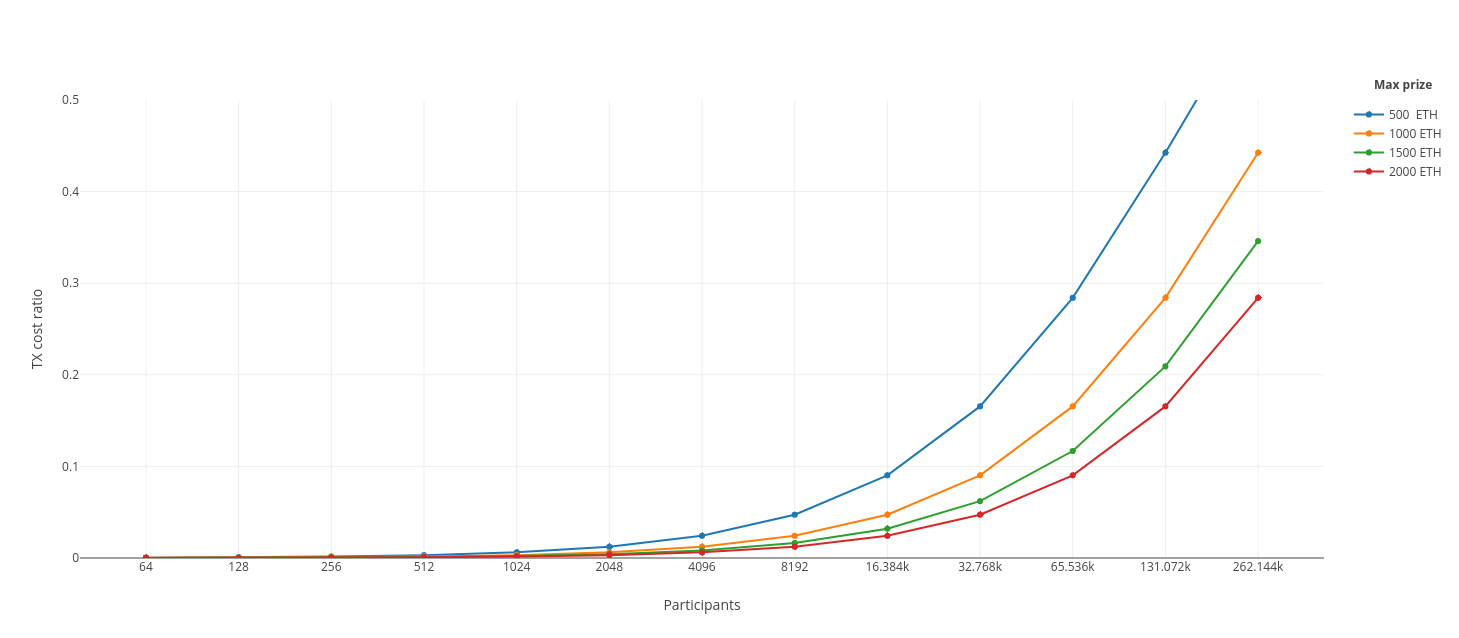
\includegraphics[width=\columnwidth]{figures/max_participants_cost_ratio.png}
  \caption{Cost ratio as a function of participants and max prize.}
  \label{fig:cost-ratio-chart}
\end{figure}

\begin{figure}[htbp]
  \centering
  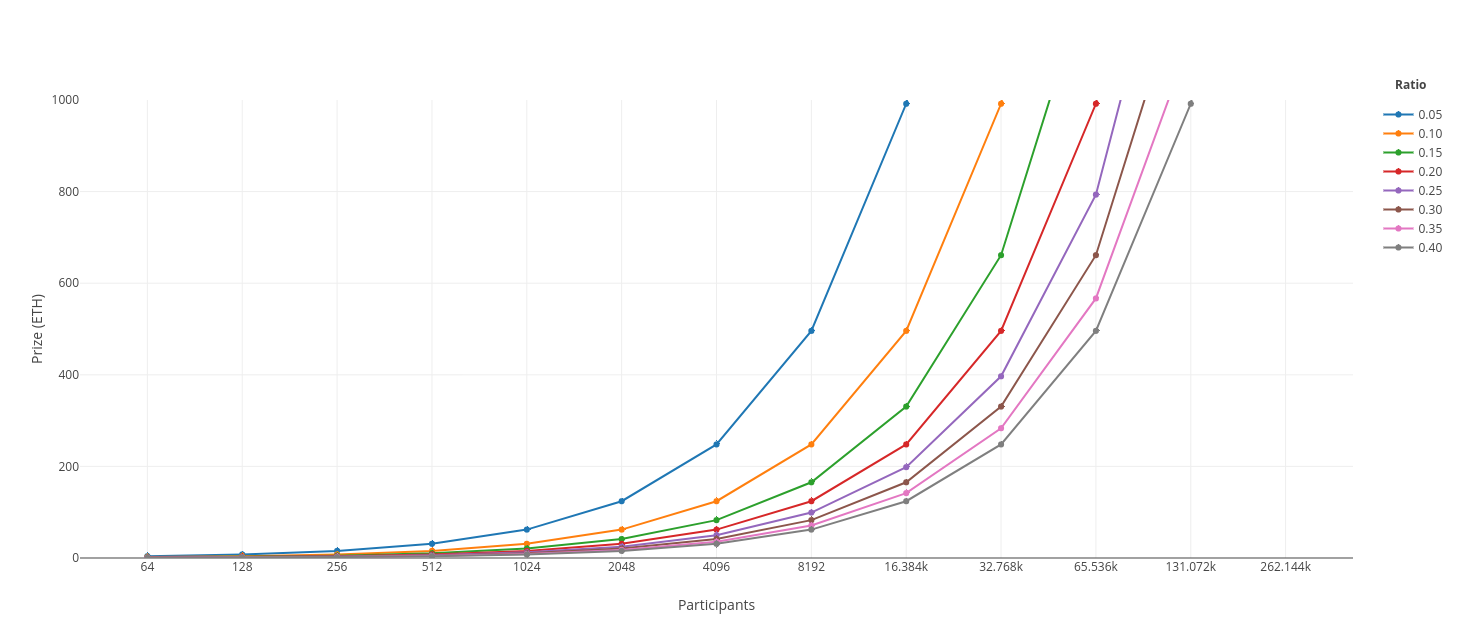
\includegraphics[width=\columnwidth]{figures/max_participants_prize.png}
  \caption{Prize as a function of participants and cost ratio.}
  \label{fig:prize-chart}
\end{figure}

\begin{figure}[htbp]
  \centering
  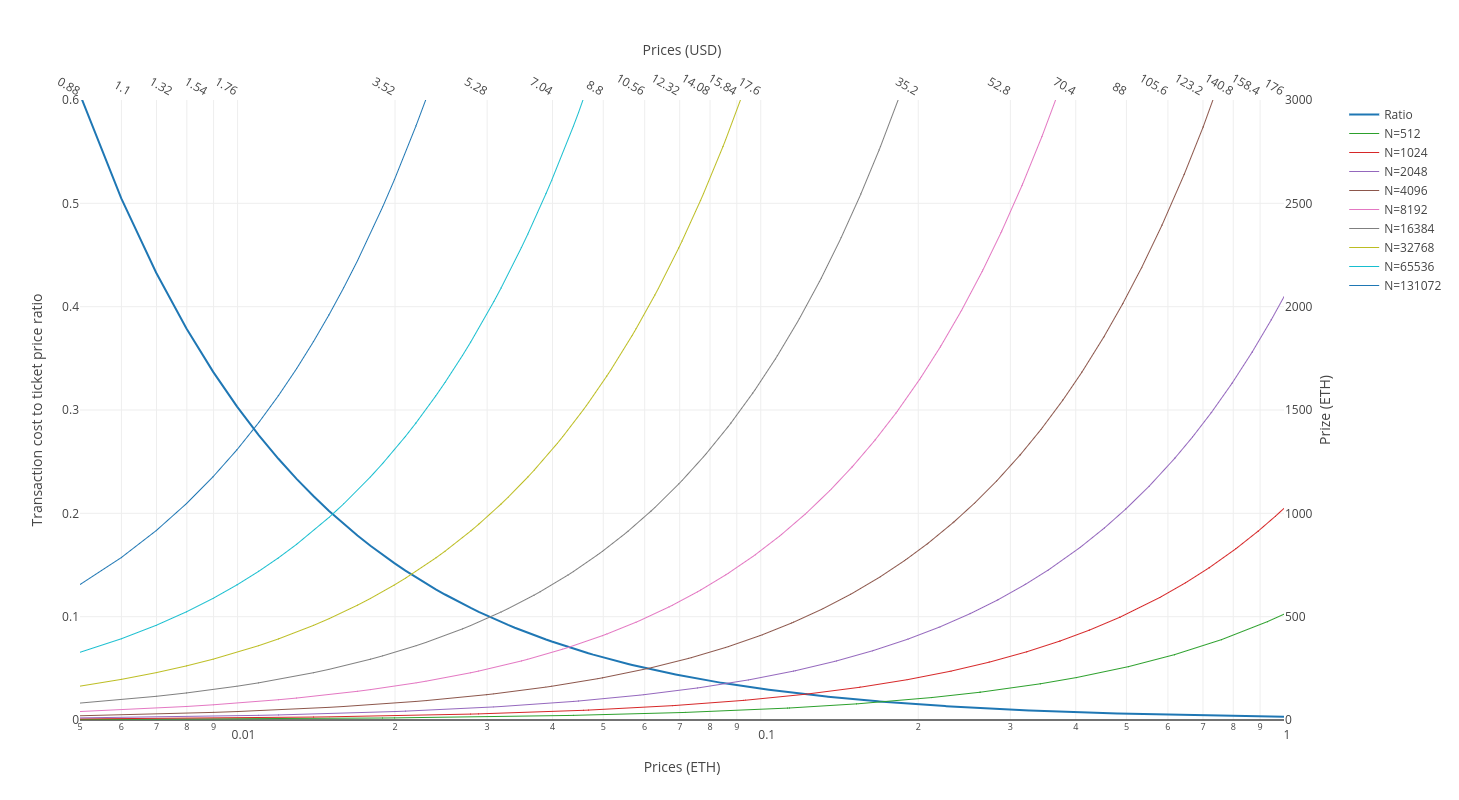
\includegraphics[width=\columnwidth]{figures/ticket_prices.png}
  \caption{Cost ratio and prize as a function of participants and ticket price.}
  \label{fig:price-chart}
\end{figure}

\section{Analysis}
\label{sec:analysis}

\subsection{Consequences of interactivity}

Based on the implementation choices of the lottery and the above results and discussion, it is possible to get an insight into important properties and trade-offs of the lottery. The lottery is interactive in that participants have to make several transactions in order to complete it successfully. The interactivity is a trade-off made in this design, as opposed to that of \cite{andrychowicz_secure_2014,bentov_how_2014}, where fewer transactions are necessary, but an upfront deposit is needed from all participants. We found that in our design, this has consequences for the scalability for several reasons. One is that the amount of transactions needed to play the lottery will be so high that it will start to congest the entire Ethereum network. Another reason is that the transaction costs put a lower bound on the minimum viable ticket price. As we operate with a maximum lottery prize for security reasons, this means that lotteries with higher ticket prices will have less capacity for participants.

What is gained by the interactivity of the scheme is that the lottery will complete as long as just one player follows the rules. Deposits are not needed as it seems a player has nothing to gain by not following the rules. A collusion of participants will not be able to predict the outcome of the randomness other than the outcome of the matches between players in the collusion. Due to secrets being committed to and not revealed until both players of a match have finalized their commitments, a collusion will not have any advantage over a single honest player.

We found that it is the cost of setting up the lottery by deploying contracts that is the most significant transaction cost. Since this cost directly influences the minimum viable ticket price, reducing the transaction cost of setting up the lottery would make the lottery capable of having more participants. It is likely that reducing the transaction cost can be done by using different design patterns in the smart contracts. Simply optimizing the length of the variables will also save some transaction costs. The current implementation only uses \texttt{uint256} types for numbers, but most of the numbers will never be so big that they need 256 bits to represent them.

The number of transactions needed to play the lottery has consequences both for the scalability of the lottery and the total transaction cost. This number can be reduced by playing the digital coin tosses \emph{off-chain}. Off-chain means that some part of a protocol is handled between the players over another communication channel than directly on the blockchain. Consider the digital coin toss after the commitments are made. As the outcome at that point is determined if both players reveal their secrets, it's not actually necessary to do that on the blockchain. The players could simply reveal their secrets to each other in private, and then one player would not have to make an actual transaction, as the losing party would not gain anything but still pay a transaction fee. If only the winner makes a reveal transaction, they will win regardless of what the loser does. Doing this requires no change in the smart contracts from what they are in the current implementation. 

It is possible that this idea of negotiating the matches off chain could be taken even further by using hierarchical deterministic secrets (HDS) \cite{wuille_bitcoin_2012}. The idea is that participants make a single commitment to a public key at the beginning of the tournament. In each match of level $i$, players derive a private key of index $i$ from the committed public key. This private key will serve as the secret in a normal digital coin toss protocol. The way HDS work is that a parent asymmetric key pair $(SK_p, PK_p)$ can generate deterministic key child key pairs with specific indices. By knowing just the public parent key, one can generate child public keys $\{PK_0, ..., PK_i\}$, and by knowing the private parent key, one can generate child private keys $\{SK_0, ..., SK_i\}$ which correspond to public keys with the same index. This means that a single public key can serve as a series of commitments by using its child public keys. The secrets will be verifiable as it is possible to verify that a private key corresponds to a public key if one knows both. Using this idea, a lottery could be negotiated off-chain once all players have made their commitments. Since it must be necessary to enforce the rules in case participants do not engage in the off-chain negotiation, all the contracts in the tournament would still have to exist, but would not necessarily be used. If commitments are made during the purchasing phase, the spike in transaction demand when playing the first matches could be drastically be reduced, hence increasing the scalability of the lottery.

\subsection{Tournament without a full binary tree}

The design of the lottery uses a tournament that is required to be a full binary tree and to be set up before players join. This limits the amounts of players in the lottery to those that is a power of two. While this limitation might make the lottery impractical, it makes it easier to reason about its properties in theory. If one were to allow for more flexible amounts of participants by allowing a non-full binary tree in the tournament, one would have to make sure that players would still have the same probability of winning. For instance, if one handles a tournament with $2^L+1$ players by having one player in a separate subtree, that player would advance to the final match without playing a single match before that. Should that player then be eligible for a smaller prize, or pay a higher ticket price?

Another possible solution is to have some matches consisting of three players instead of just two. Unfortunately, due to the time limits, this can give an advantage to two players in the same match colluding. In a match with three players, each player would ideally have a $\frac{1}{3}$ probability of winning, so that in a match with two colluding players, they would have a $\frac{2}{3}$ probability of winning. But if the secret of the non-colluding party Alice is revealed first, the colluding parties Colin and Lucy have three options. (i) Only Colin reveals, (ii) only Lucy reveals, and (iii) both reveal. Assuming each player who reveal has an equal probability of winning and that their secrets are uniformly random, the first two options each have a $\frac{1}{2}$ probability of either Colin or Lucy winning, while in the third options there's a $\frac{2}{3}$ chance of either winning. The slim probability that Alice wins in all the three options is just $\frac{1}{2 \cdot 2 \cdot 3}=\frac{1}{12}$, making the either Carol or Lucy win in 11 of 12 cases.

It is possible that there is a design in which a tournament with any amount of participants can be played fairly, but it would involve some considerable design changes from our lottery that is beyond the scope of this thesis.

\subsection{Mitigating a censorship attack}
\todo{It might be too hard to do something about this, actually.}

A possible vulnerability in censorship of transactions was discovered. Even though the risk of a censorship attack is unknown, if we assume the possibility of a miner or collusion of miners with a majority hashing power, it would at some size of the lottery prize be in their economic interest to launch such an attack. A censorship attack is possible because of the time limits of matches, because a player unable to make transactions will lose. The time limits are however necessary to prevent a single participant halting the entire process. 

A possible way of mitigating a censorship attack is to annul the result of the tournament if the winner won a certain fraction of their matches by forfeiture. This could possibly do some collateral damage in that an honest winner could risk being suspected of cheating. It could also make the off-chain negotiation mentioned earlier in this section impractical. 
